\chapter{Statistical methods}\label{ch:statistic}

Gluck, Harris and Prado, in the original BREACH paper, investigated the attack
on stream ciphers, such as RC4. They also suggested that block ciphers are
vulnerable, without providing practical attack details. However, the use of RC4
is also prohibited in negotiation between servers and clients
\cite{rc4_prohibit} due to several other major vulnerabilities.

In this paper we perform practical attacks against popular block ciphers, by
using statistical methods to by-pass noise created from random portions of data
stream, padding or the Huffman coding. Also, we propose various optimization
techniques that can make the attack much more efficient.

\section{Probabilistic techniques}\label{sec:probabilistic}

Block ciphers provide a greater challenge compared to stream ciphers, when it
comes to telling length apart, since stream ciphers provide better granularity.
In this work we use statistical techniques to overcome this problem.

Furthermore, Huffman coding may affect the length of the compressed data stream,
since the character frequency might be affected, resulting to different Huffman
tables and subsequently different length. We will also propose a method to
bypass Huffman induced noise.

\subsection{Attack on block ciphers}

Block ciphers are the most common used ciphers in modern websites. Especially
AES \cite{aes} is used in major websites such as
Facebook\footnote{\url{https://www.facebook.com}},
Google\footnote{\url{https://www.google.com}},
Twitter\footnote{\url{https://www.twitter.com}},
Wikipedia\footnote{\url{https://www.wikipedia.org}},
YouTube\footnote{\url{https://www.youtube.com}},
Amazon\footnote{\url{https://www.amazon.com}} and others. In this paper we
introduce methods to attack such block ciphers, using the attack model described
in Chapter \ref{ch:attack}.

First of all, a packet stream of a specific endpoint needs to be examined, in
order to find patterns and better understand the distribution of the data stream
on TLS records and TCP packets. In the following figures two request streams can
be seen, for Facebook Touch and Gmail respectively.

\begin{figure}[H] \caption{Facebook flow} \centering
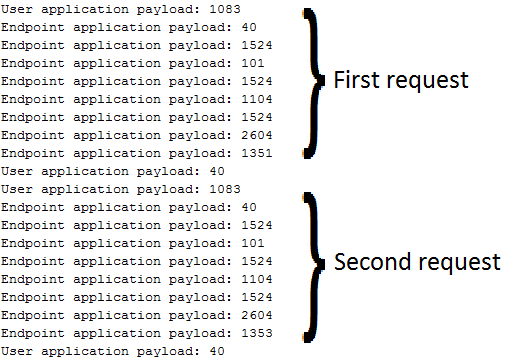
\includegraphics[width=0.6\textwidth]{diagrams/facebook_request_flow.png}\end{figure}

\begin{figure}[H] \caption{Gmail flow} \centering
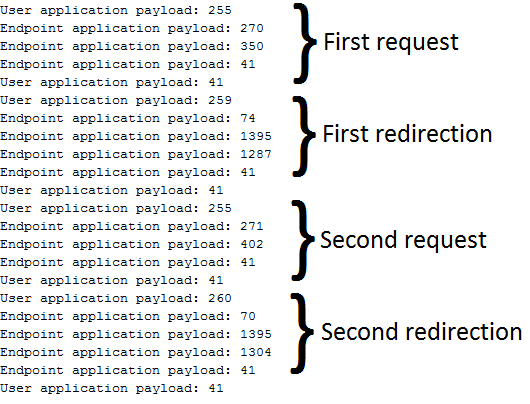
\includegraphics[width=0.6\textwidth]{diagrams/gmail_request_flow.png}\end{figure}

A close look on the above record stream reveals interesting information about
the pattern multiple requests on the same endpoint present.

Specifically, the first figure shows two consequent requests on the search
method of Facebook Touch. The two requests were issued under the attack context
and it can be seen that they differ only in a single TLS record, regarding the
record lengths.

At this point it would be safe to assume that the specific record, that differs
in the two requests, is the one containing the attacker's chosen plaintext. In
order to confirm this, mitmproxy can again be used along with the MitM proxy we
have developed.

Mitmproxy uses netlib\footnote{\url{https://pypi.python.org/pypi/netlib}} as a
data-link library. Netlib's \texttt{read\_chunked} function performs the reading
of the TLS record fragments. We added \texttt{print} markers in this function,
which mark the log that contains the packet flow passing through our MitM proxy
and also provides the sectors that the plaintext is divided before compression.
Comparing the log with the decrypted, decompressed chunks of plaintext we have
confirmed that the sector of the plaintext that contains the reflection is
contained in the TLS record that differs in the length flow.

The above flows lead to another interesting deduction. If the implementation of
the block cipher was as expected, each record should have been of length that is
a product of 128 bits and, consequently, the two records that differ should have
had the same length or differ on a product of 128 bits also.  However, that is
not the case here.

In order to further investigate the implementation of block ciphers, we have
issued the attack on multiple operating systems, networks and browsers. The
parameter that seemed to demonstrate similar behaviour on these cases was the
browser, as for different OSs and networks the packet flow was structurally the
same for the same browser version.

In the following figures we present two distinct packet flow structures that
were observed during the experiments on different browsers and versions.

\begin{figure}[H] \caption{Older browser version} \centering
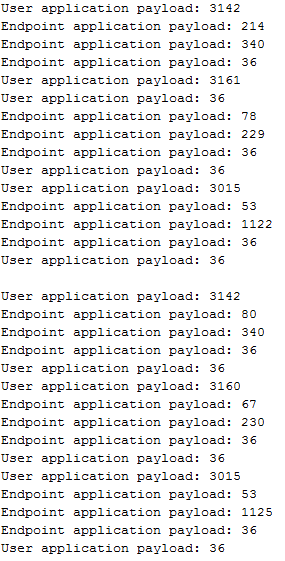
\includegraphics[width=0.4\textwidth]{diagrams/older_browser_version.png}\end{figure}

\begin{figure}[H] \caption{Newer browser version} \centering
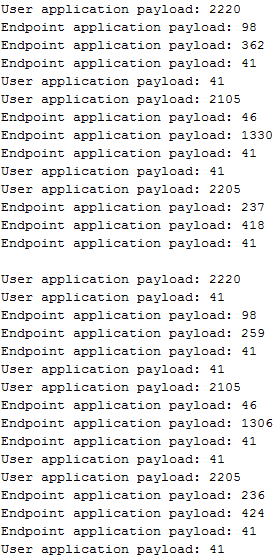
\includegraphics[width=0.4\textwidth]{diagrams/newer_browser_version.png}\end{figure}

In older browser versions, the packet that contains the reflection is the one
with length 1122 for the first request and 1125 for the second request.  Each
request of the flow showed a difference of a few bytes, that would not exceed 20
at any time. In newer versions of browsers, the packet that contains the
reflection is of length 418 for the first request and 424 for the second. In
other cases, the difference could be tens or hundreds of bytes for two requests.

Browsers that were used, Mozilla Firefox, Google Chrome, Chromium and Iceweasel,
all use Mozilla's Network Security Services (NSS)
library\footnote{\url{https://developer.mozilla.org/en-US/docs/Mozilla/Projects/NSS}}
for the implementation of TLS. Following the above discoveries, we have found
that the first pattern was demonstrated in browser versions that used NSS
3.17.3 release or older, whereas the second pattern was demonstrated on
browsers that used newer NSS releases. Since that release fixed \texttt{Bug
1064670}\footnote{\url{https://bugzilla.mozilla.org/show_bug.cgi?id=1064670}},
we could wildly assume that it was that bug that was responsible for that
behaviour.  However, further investigation needs to be done, in order to
determine why the block cipher implementation does not follow the
theoretical standards.

In any case, the above patterns allow us to use statistical methods to extract
conclusions regarding the length. Specifically, by issuing hundreds or thousands
of requests for the same string and calculating the mean length of the
responses, the correct symbol should converge in a smaller mean length that an
incorrect. This method also allows us to bypass noise introduced by random
strings in the HTML body.

\subsection{Huffman fixed-point}

Huffman coding, as described in Section \ref{subsec:huffman}, uses letter
frequency in order to produce a lossless compression of the data stream. By
inserting a chosen plaintext in the data stream, the attacker would affect this
frequency, probably resulting in differentiated Huffman table and affecting the
length of the compressed stream altogether.

In this section we will describe a methodology to bypass the noise induced by
Huffman coding. In particular, we present a way for two different requests, in
the same stage of the attack, to demonstrate the same letter frequencies, so
that the attack itself does not affect the Huffman table of the compression.

Initially, an alphabet pool is created, containing every item of the alphabet
that the secret belongs to. The key point lies in the fact that Huffman coding
does not take into account the position of the characters, only the frequency of
appearance for each one.

So, if, for instance, the alphabet is made up of decimal digits, two different
requests can be crafted as below:

\begin{figure}[H] \caption{Huffman fixed-point.} \centering
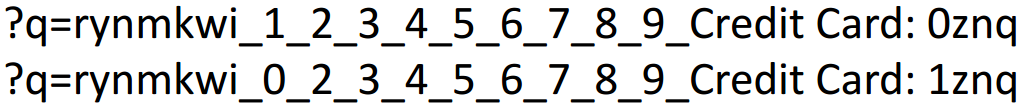
\includegraphics[width=0.8\textwidth]{diagrams/huffman_fixed_point.png}\end{figure}

As can be seen, the frequency of each letter is not affected from one request to
another, whereas rearranging the position allows us to perform the attack.

The above figure also depicts the use of random nonces before and after the main
body of the request, in this case \texttt{rynmkwi} and \texttt{znq}
respectively. These nonces are used to avoid the Huffman fixed-point prefix or
the character tested to be LZ77 compressed with strings before, in this case
\texttt{?q=}, or after the request, and affect the consistency of the tests.

Our implementation of the methodology described is found in the request
initialization library \ref{sec:hillclimbing_py}. A user needs to input a chosen
prefix for the bootstrapping and an alphabet pool from some predefined alphabets
- uppercase letters, lowercase letters, decimal digits and dashes - as well as
serial or parallel method of attack - serial is chosen by default. The
functions of the library will then create the appropriate request file, that
can be used along with the BREACH script to issue the attack.

\section{Attack optimization}\label{sec:optimization}

The previous chapters have focused on expanding and explaining how the attack
could be a viable threat in real world applications. However, work still needs
to be done to make it faster and minimize the margin of error.

In this section we will describe two methods that improve the performance of the
attack, parallelization of hill-climbing and cross-domain parallelization.

\subsection{Parallelization of hill-climbing}

Up to this point, the characters of the alphabet are tested serially, one after
the other and again from top, when the end of the alphabet is reached.  However,
a more efficient method could be followed, that could reduce the time of the
attack from \begin{math}O(|S|)\end{math} to \begin{math}O(log|S|)\end{math}.

The idea behind this method is based on the well-known
\texttt{divide-and-conquer} paradigm. Specifically, instead of using one test
character each time, concatenated with the known prefix, we could divide the
alphabet pool in half and issue requests on each such half. A request file
parameterized as such is the following:

\plaintext{File with parallelized request parameters.}{parallel_request.txt}

Using this method, for each step of the attack two different requests are made.
The first corresponds to one half of the alphabet and the second to the other
half. Whichever minimizes the length function is safe to assume that contains
the correct secret, so it is chosen and the same method applies to it, until a
single character is chosen. That way we use binary searching techniques,
dropping the attack factor noticeably.

The conditions for Huffman-induced noise and collateral compression are also met
here, using the alphabet pool and the random nonces. Also, in case of combined
alphabets, such as lowercase letters, uppercase letters and digits, it could be
possible that biases were introduced regarding the different types, i.e.
lowercase letters could be better compressed than uppercase ones. We also bypass
this issue by dividing the alphabet alternately, instead of consecutively.

\subsection{Cross-domain parallelization}

The tree structure of the Domain Name System
(DNS)\footnote{\url{https://en.wikipedia.org/wiki/Domain_Name_System}} defines
each non-resource record node as being a domain name. Each domain that is part
of a larger domain is called subdomain. Most websites use subdomains for
specific applications, that hold a certain role in the context of the basic web
application. Such applications include language versions of the website, mobile
versions or divisions of a larger organization, such as Schools in a University.

The existence of different subdomains can be used in the context of the attack
to make it more efficient. In that case, multiple subdomains should handle same
or similar data containing the chosen secret. If cookies are available on the
parent domain, they are also available in the subdomains and can be used from
the attacker.

Specifically, via DNS poisoning, different subdomains can resolve to different
IPs. The source and destination IP information is included in the Transport
Layer of the network, so it can be seen by an eavesdropper or, in our case, the
MitM proxy. The attack can be then issued on both domains, effectively
parallelizing it with up to Nx efficiency, where N is the number of different
domains and subdomains.
